\documentclass[UTF8,oneside]{ctexbook}

% \usepackage[utf8]{inputenc} %指定编码方式为utf8
\usepackage[titles]{tocloft} % 目录
% \usepackage{fancyhdr} % 页眉页脚
% \pagestyle{fancy} % 美化页眉
%\usepackage{appendix}
\usepackage{graphicx} % An example of a floating figure using the graphicx package.
\usepackage{animate} % 动画
\usepackage[caption=true, font=footnotesize]{subfig}% 前面的[]为了防止覆盖IEEE默认选项
\usepackage{float} %禁止浮动
\usepackage{enumerate} % 列表
\usepackage{xpinyin} % 注音
\usepackage{amsmath} % 数学
\usepackage{listings} %抄录环境
\usepackage{color} %定义颜色
\definecolor{codegreen}{rgb}{0,0.6,0}
\definecolor{codegray}{rgb}{0.5,0.5,0.5}
\definecolor{codepurple}{rgb}{0.58,0,0.82}
\definecolor{backcolour}{rgb}{0.95,0.95,0.92}

\usepackage[colorlinks,linkcolor=blue]{hyperref} % 超链接
\usepackage[margin=3cm]{geometry} % 更改页边距


\title{\Huge{在Github上团队协作}\\
\large{V1.0}}
\author{\href{https://github.com/lonelybag?tab=repositories}{\Large{@LonelyBag}}\\ {\itshape \large{Edite by \href{https://mirrors.tuna.tsinghua.edu.cn/CTAN/systems/texlive/Images/}{\LaTeX}}}}

\begin{document}
% ----------- 封面 ---------------
\frontmatter
\maketitle

\begin{center}  % 居中
	\quad \\
	\vspace{5cm}
	\LARGE{真正的勇气不在于取人性命,而在于恕人罪恶}\\
\end{center}
\thispagestyle{empty}

\clearpage
\begin{center}  % 居中
	\quad \\
    \vspace{5cm}
    \LARGE{联系方式}\\
	\LARGE{E-mail:dongweihao\_dreamer@163.com}\\
	\href{https://www.zhihu.com/people/lonelybag-79/activities}{LonelyBag的知乎}\\
	\href{https://github.com/lonelybag?tab=repositories}{LonelyBag的Github}
\end{center}
\thispagestyle{empty}

% ----------- 目录 ---------------
\tableofcontents
\mainmatter
%--------- 定义代码抄录格式 -------
\lstset{
	backgroundcolor=\color{backcolour},
	commentstyle=\color{codegreen},
	keywordstyle=\color{magenta},
	numberstyle=\tiny\color{codegray},
	stringstyle=\color{codepurple},
	basicstyle=\footnotesize,
	breakatwhitespace=false,
	breaklines=true, % 允许断行                 
	captionpos=b,
	keepspaces=true,
	numbers=none,
	numbersep=5pt,
	showspaces=false,
	showstringspaces=false,
	showtabs=false,
	tabsize=2
}
% \iffalse \section{========= 不编译 开 =========}
% \section{========= 不编译 关 =========}\fi
% \section{========= 结束 =========}\end{document}
\chapter{用Github提交Issues}
\section{什么是Issues?}
举个例子,这是\LaTeX 中文论坛在Github上维护的一个\href{https://github.com/latexstudio/LaTeXPackages-CN}{项目},它的Issues是这样的
\begin{figure}[H]
	\centering
	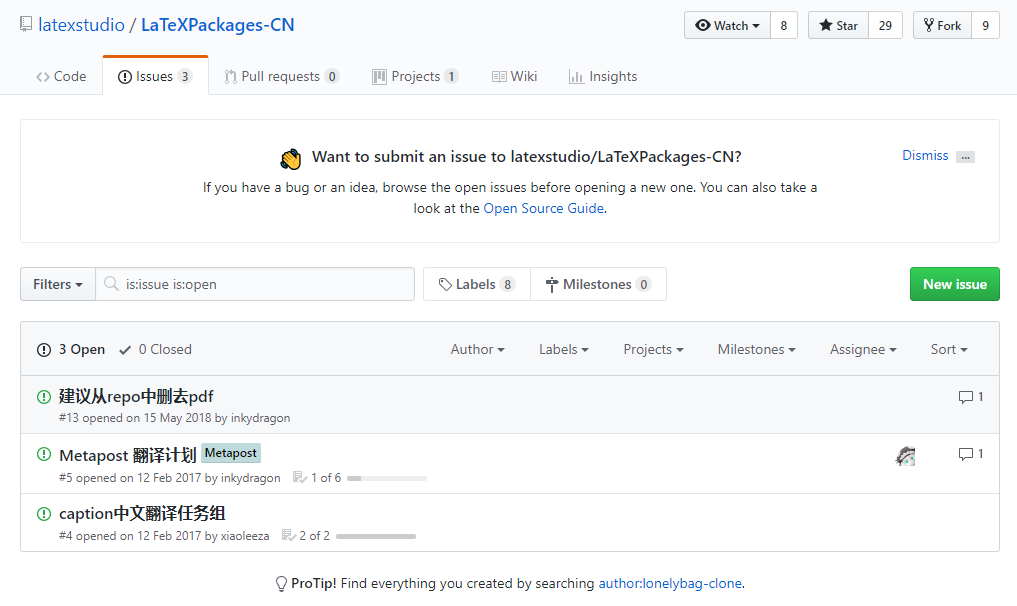
\includegraphics[width=1\linewidth]{Pics/latexcn.png}
	\vspace{-0.3cm}
	\caption{一个例子}\label{fig:latexcn}
\end{figure}

我们点开第一个看一下
\begin{figure}[H]
	\centering
	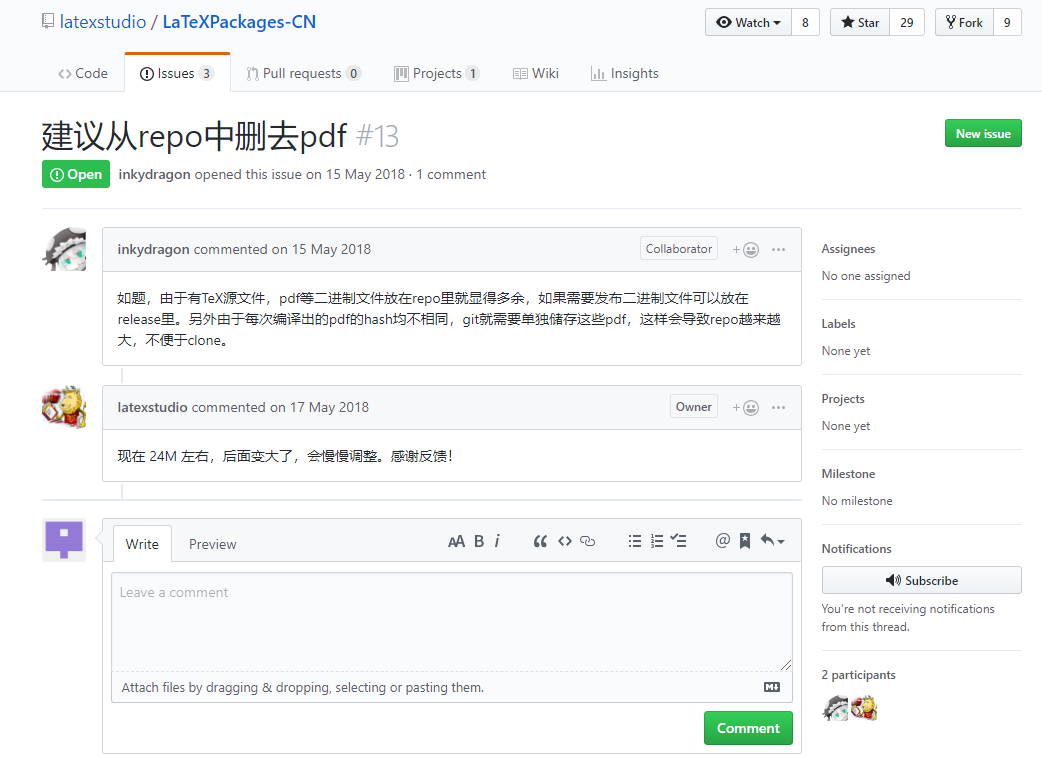
\includegraphics[width=1\linewidth]{Pics/latexcn2.png}
	\vspace{-0.3cm}
	\caption{第一个issue}\label{fig:latexcn1}
\end{figure}

可以看出这个issue是为了改进项目而提出的,我们再打开第二个issue
\begin{figure}[H]
	\centering
	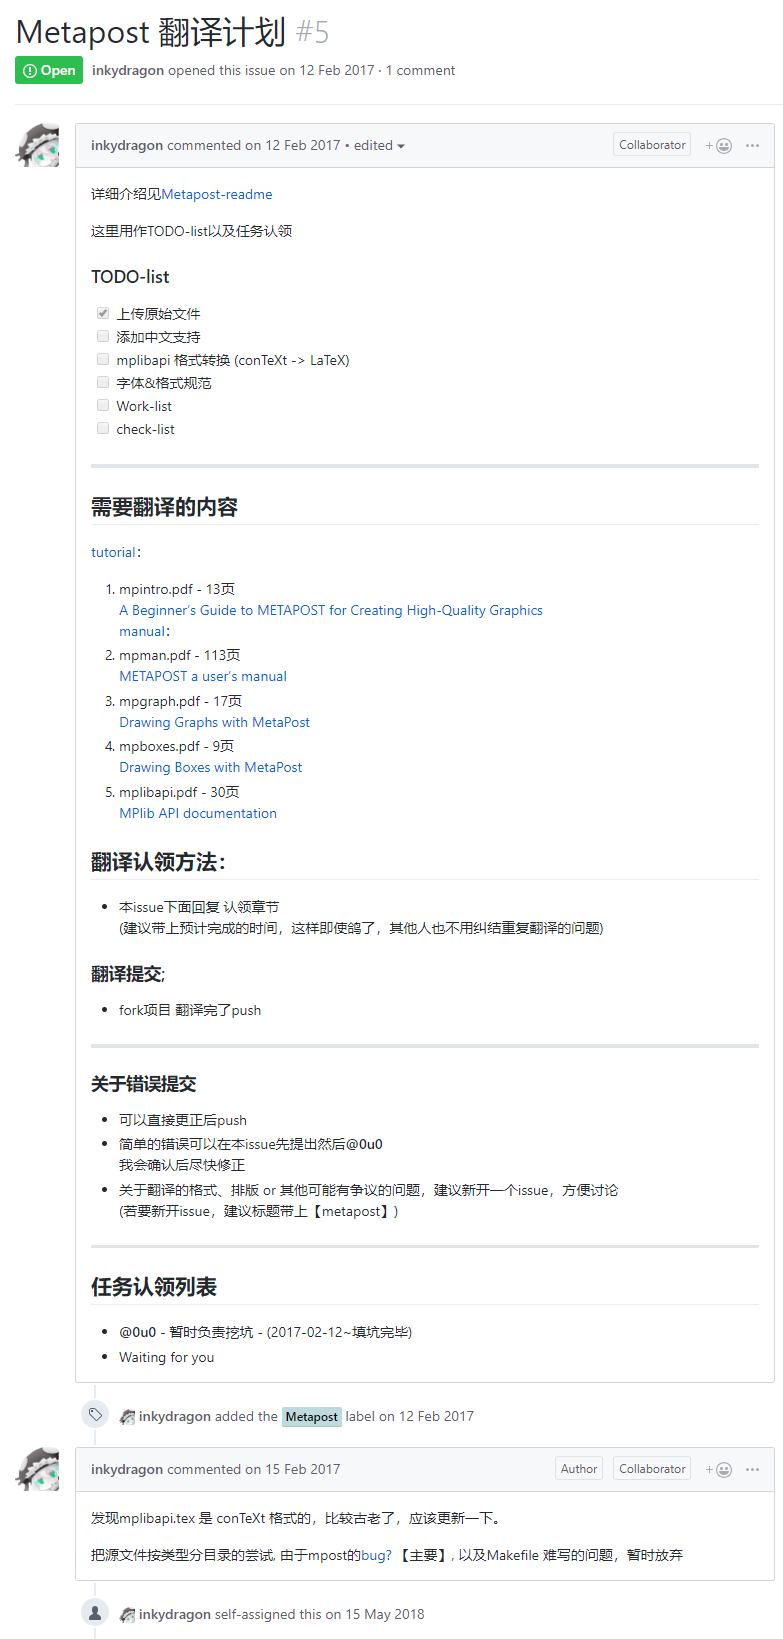
\includegraphics[width=0.6\linewidth]{Pics/latexcn3.png}
	\vspace{-0.3cm}
	\caption{第二个issue}\label{fig:latexcn1}
\end{figure}

这个issue为项目成员分配了任务并列出了一个任务清单。

此外大家还可以看一下其他项目的issue,如:\href{https://github.com/jikexueyuanwiki/tensorflow-zh/issues}{谷歌TensorFlow官方文档中文版}以及\href{https://github.com/llSourcell/YOLO_Object_Detection/issues}{YOLO Object Detection},也有一些有趣的issue,比如:\href{https://github.com/geekyouth/geekyouth.github.io/issues}{用issue写博客},以及\href{https://github.com/sindresorhus/ama/issues/2}{晒猫的?}。。。

我个人认为issue的主要任务是提交BUG,这种类似于知乎的“提问 - 回答”的形式为所有用户提供了一个开放平台用于提交项目中的问题,很方便、透明,建议读者也使用这种形式进行协作。

\section{如何提交issue}
以\href{https://github.com/lonelybag?tab=repositories}{\Large{LonelyBag}}建立的项目为例,解释普通用户如何提交issue。

首先,打开这个\href{https://github.com/lonelybag/Latex_lonelybag}{repo}\footnote{全称repository,在github中表示一个项目,如:\href{https://github.com/lonelybag/git-flight-rules/blob/master/README_zh-CN.md}{Git教程}。}。

然后点击issue按钮,如图\ref{fig:issue1}所示。
\begin{figure}[H]
	\centering
	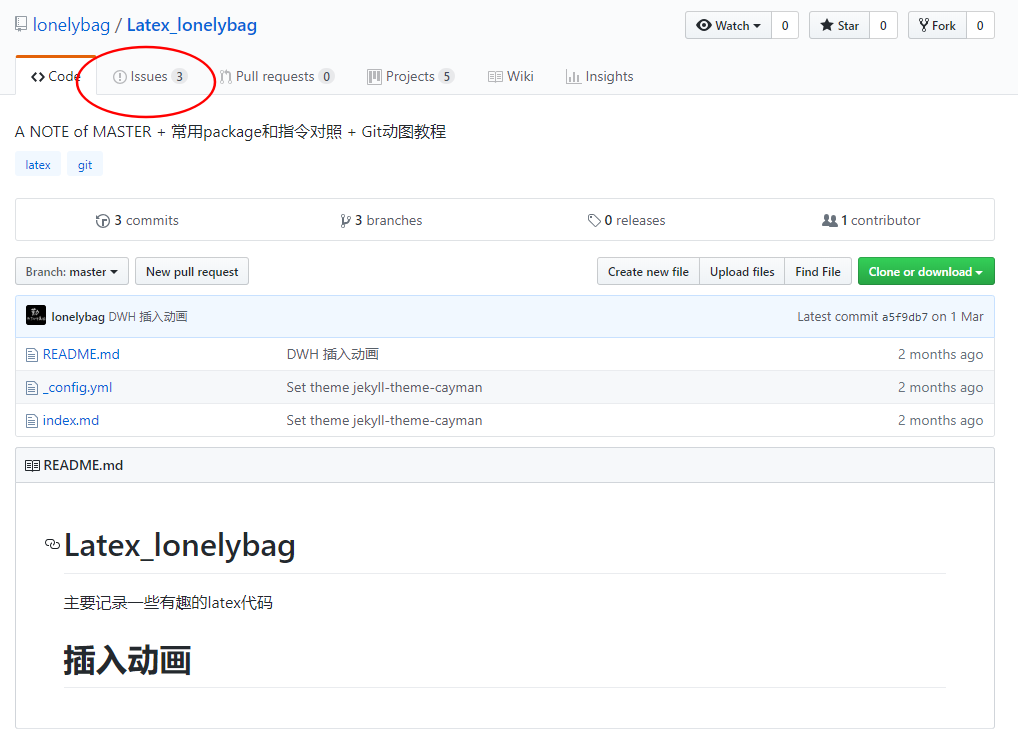
\includegraphics[width=0.6\linewidth]{Pics/issue1.png}
	\vspace{-0.3cm}
	\caption{issue按钮}\label{fig:issue1}
\end{figure}

可以看见共有三个issue,让我们点击New issue按钮。
\begin{figure}[H]
	\centering
	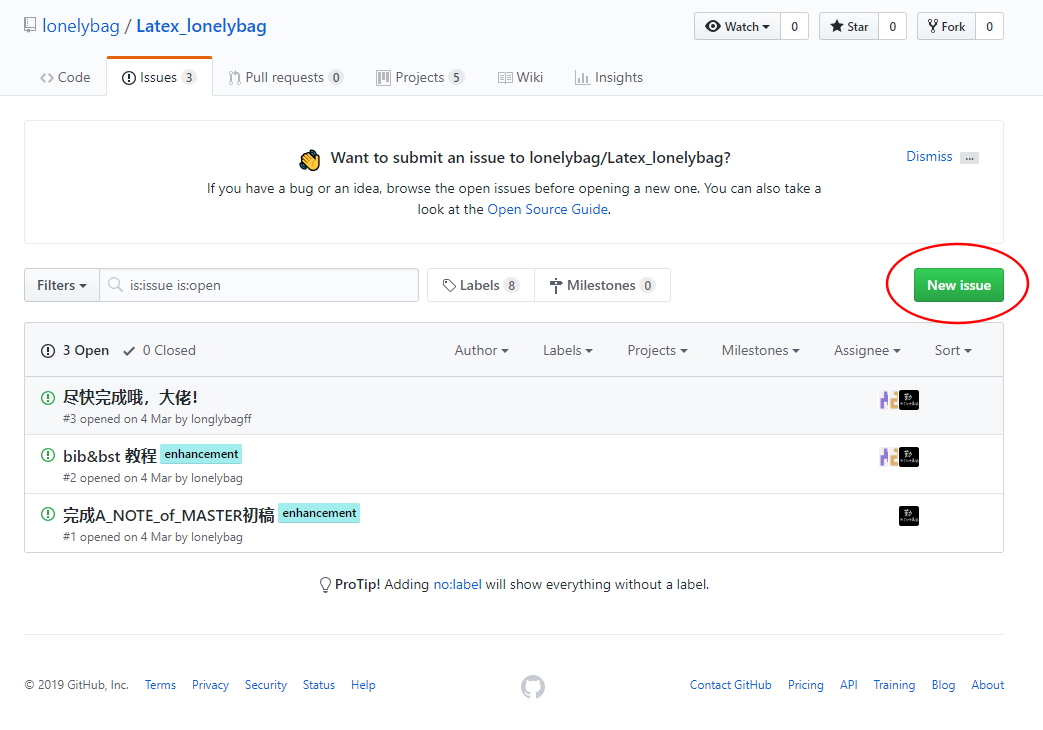
\includegraphics[width=0.6\linewidth]{Pics/issue2.png}
	\vspace{-0.3cm}
	\caption{New issue按钮}\label{fig:issue2}
\end{figure}

可以看到在这里需要填写标题和内容,编辑框中支持Markdown语言(一种用来编辑弱格式、强框架文档的语言),红框中是一个官方文档。
\begin{figure}[H]
	\centering
	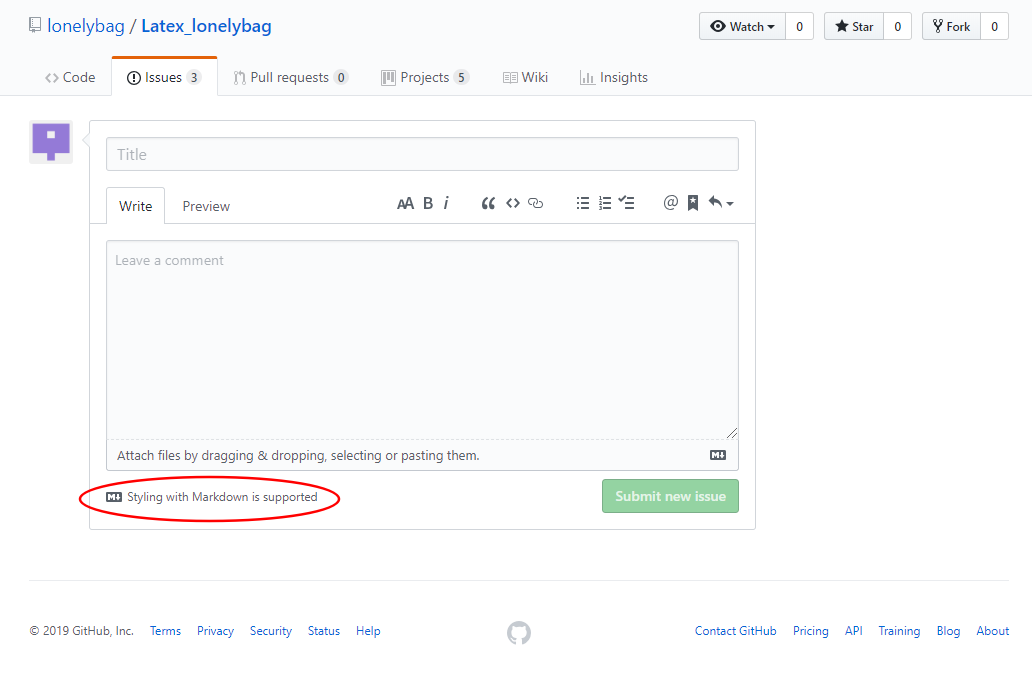
\includegraphics[width=0.6\linewidth]{Pics/issue3.png}
	\vspace{-0.3cm}
	\caption{编辑issue}\label{fig:issue3}
\end{figure}

试着输入一些内容(箭头指的位置表示我们可以将图片直接拖拽到这里并上传)
\begin{figure}[H]
	\centering
	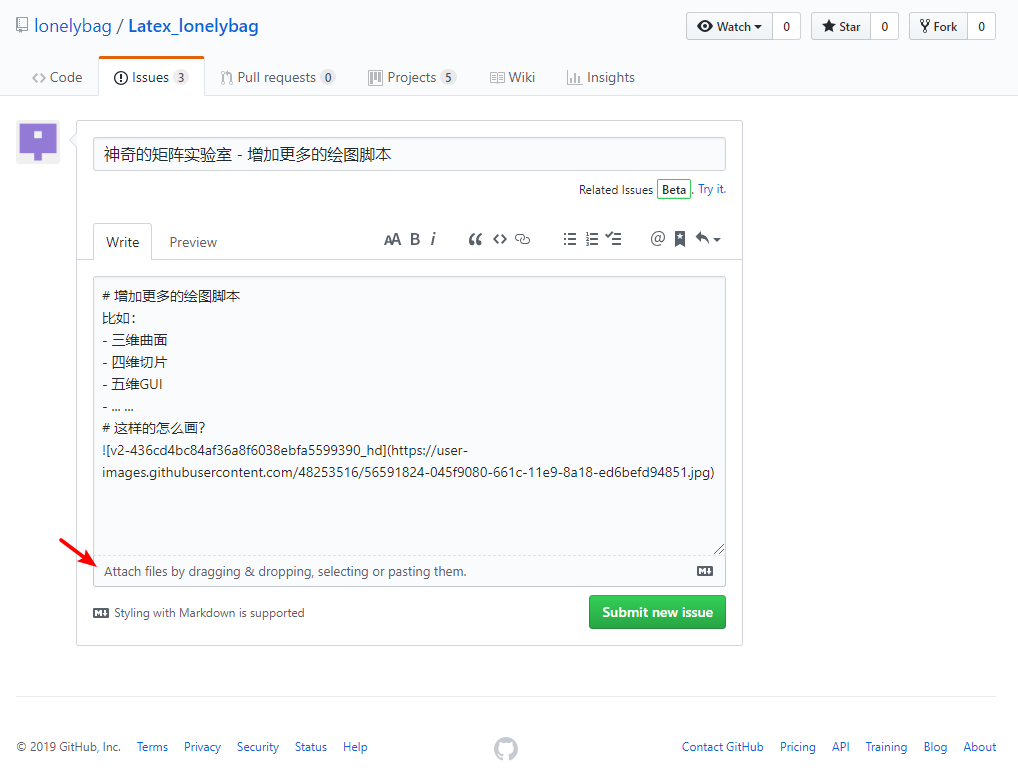
\includegraphics[width=0.6\linewidth]{Pics/issue4.png}
	\vspace{-0.3cm}
	\caption{输入一些内容}\label{fig:issue4}
\end{figure}

还可以预览一下效果
\begin{figure}[H]
	\centering
	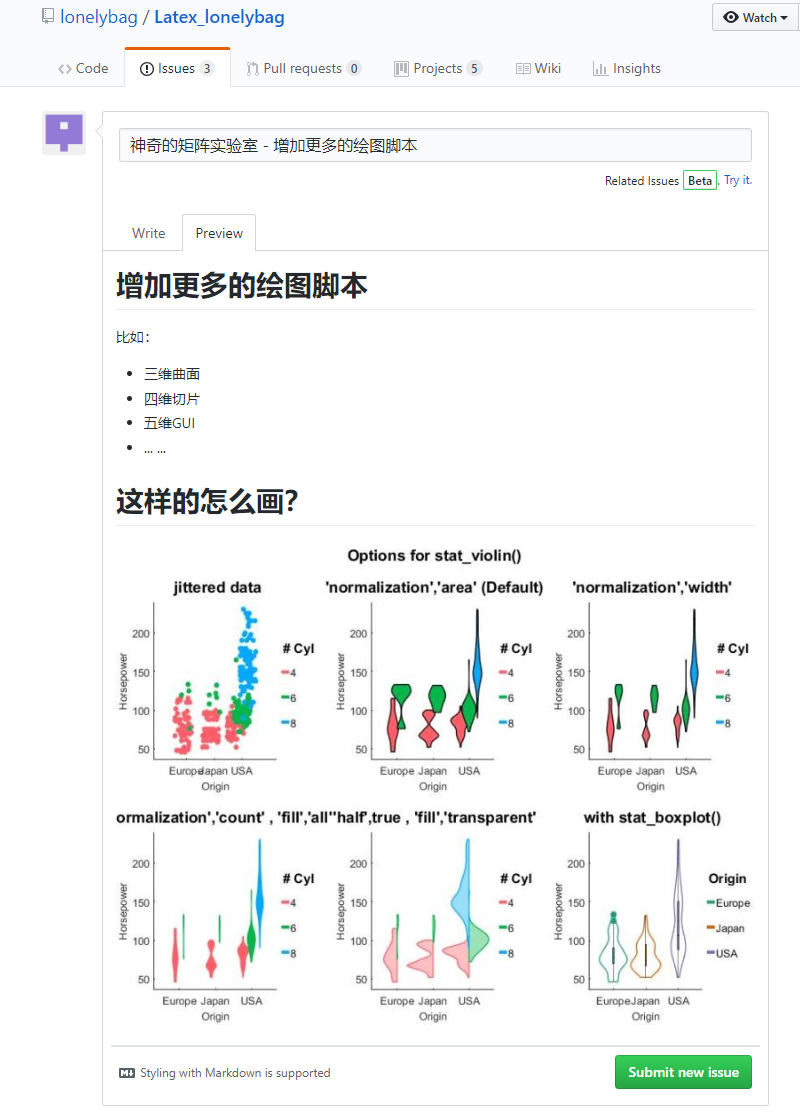
\includegraphics[width=0.6\linewidth]{Pics/issue5.png}
	\vspace{-0.3cm}
	\caption{预览内容}\label{fig:issue5}
\end{figure}

满意后就可以提交了,注意到提交后依然可以继续添加评论。
\begin{figure}[H]
	\centering
	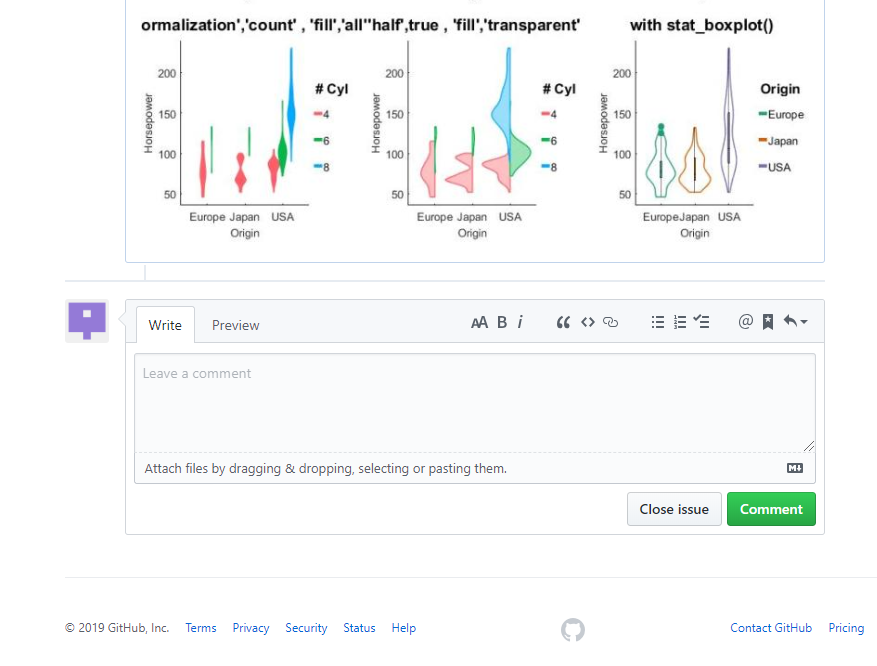
\includegraphics[width=0.6\linewidth]{Pics/issue6.png}
	\vspace{-0.3cm}
	\caption{预览内容}\label{fig:issue6}
\end{figure}

需要注意的是,项目作者以及issue作者均可以关闭或重新打开这个issue,但是其他人只能添加和删除comment,如图所示。
\begin{figure}[H]
	\centering
	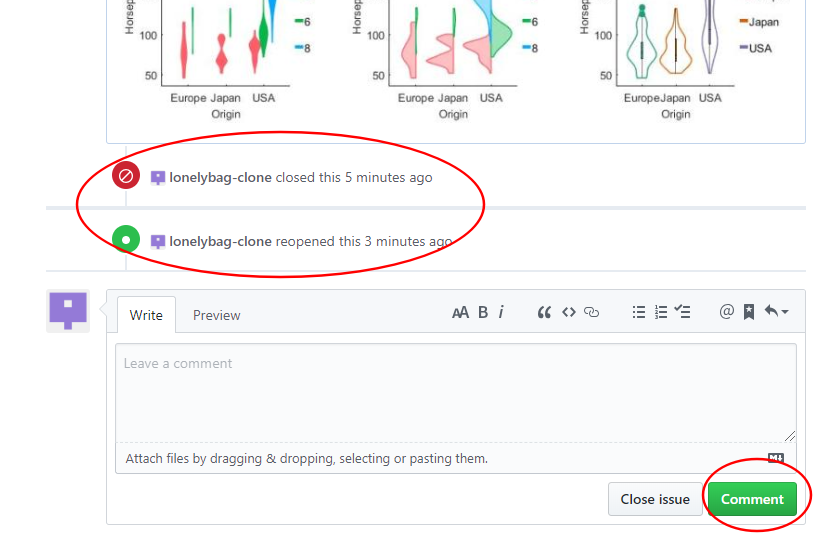
\includegraphics[width=0.6\linewidth]{Pics/issue7.png}
	\vspace{-0.3cm}
    \caption{提交issue作者的关闭issue按钮可见}\label{fig:issue7}
\end{figure}

这样就完成了普通用户的issue提交和评论,接下来我切换到项目负责人的账号中看看其中会发生什么。
\begin{figure}[H]
	\centering
	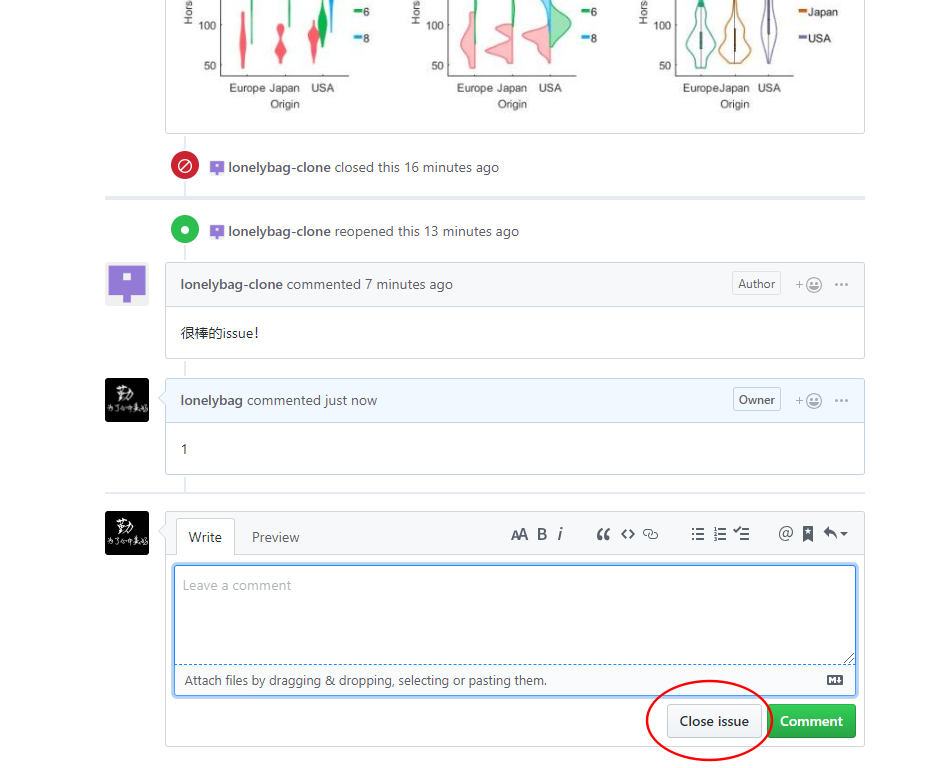
\includegraphics[width=0.6\linewidth]{Pics/issue8.png}
	\vspace{-0.3cm}
	\caption{项目负责人的关闭issue按钮可见}\label{fig:issue8}
\end{figure}
可以看出,项目负责人中也可以关闭issue甚至评论。

当相应BUG被修正或者相关功能被添加后就可以关闭issue了,而且一般会打上Tag,如下图所示。
\begin{figure}[H]
	\centering
	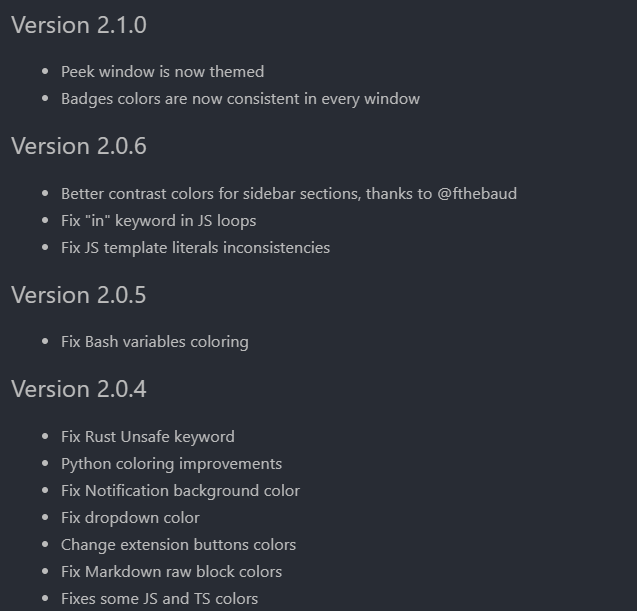
\includegraphics[width=0.6\linewidth]{Pics/issue9.png}
	\vspace{-0.3cm}
	\caption{根据issue撰写的文档}\label{fig:issue9}
\end{figure}

\chapter{如何进行团队协作}
\section{什么是Git}
\section{为什么Git}
\section{小明的一天}
\end{document}
